\hypertarget{singleton_8cpp}{
\section{src/singleton.cpp File Reference}
\label{singleton_8cpp}\index{src/singleton.cpp@{src/singleton.cpp}}
}
Implementation du design pattern singleton.  


{\tt \#include $<$iostream$>$}\par
{\tt \#include \char`\"{}singleton.hpp\char`\"{}}\par


Include dependency graph for singleton.cpp:\nopagebreak
\begin{figure}[H]
\begin{center}
\leavevmode
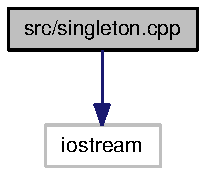
\includegraphics[width=67pt]{singleton_8cpp__incl}
\end{center}
\end{figure}


\subsection{Detailed Description}
Implementation du design pattern singleton. 

\begin{Desc}
\item[Author:]GDD \end{Desc}
\begin{Desc}
\item[Version:]0.1 \end{Desc}
\begin{Desc}
\item[Date:]29 mars 2009\end{Desc}
Implementation du design pattern singleton pour rendre une classe instanciable une unique fois. 